% !TeX root = synopsis.tex
\documentclass[10pt,a4paper]{report}

\usepackage[margin=0.75in]{geometry}
\usepackage{setspace}
\usepackage{graphicx}
\usepackage{booktabs}
\usepackage{tabularx}
\usepackage{longtable}
\usepackage{array}
\usepackage{amsmath}
\usepackage{xcolor}
\pagecolor{white}
\usepackage{enumitem}
\usepackage{tikz}
\usepackage{xurl}
\usepackage[T1]{fontenc}
\usepackage{lmodern}
\usepackage[hidelinks]{hyperref}
\usetikzlibrary{arrows.meta,positioning,shapes.geometric,fit,calc}

% Compact chapter heading styling to optimize academic proposal length (15-20 pages)
\makeatletter
\def\@makechapterhead#1{%
  \vspace*{8\p@}%
  {\parindent \z@ \raggedright \normalfont
    \ifnum \c@secnumdepth >\m@ne
        \large\bfseries \color{green} \@chapapp\space \thechapter
        \par\nobreak
        \vskip 4\p@
    \fi
    \interlinepenalty\@M
    \LARGE \bfseries \color{ink} #1\par\nobreak
    \vskip 12\p@
  }}
\def\@makeschapterhead#1{%
  \vspace*{8\p@}%
  {\parindent \z@ \raggedright \normalfont
    \interlinepenalty\@M
    \LARGE \bfseries \color{ink} #1\par\nobreak
    \vskip 12\p@
  }}
\makeatother

\setstretch{1.0}
\setlength{\parindent}{0pt}
\setlength{\parskip}{0.25em}
\setlist{nosep,leftmargin=*}
\renewcommand{\arraystretch}{1.05}
\newcolumntype{Y}{>{\raggedright\arraybackslash}X}
\newcolumntype{P}[1]{>{\raggedright\arraybackslash}p{#1}}

% Float adjustment to keep diagrams embedded with text
\renewcommand{\topfraction}{0.85}
\renewcommand{\bottomfraction}{0.85}
\renewcommand{\textfraction}{0.15}
\renewcommand{\floatpagefraction}{0.75}

\definecolor{ink}{HTML}{24343A}
\definecolor{green}{HTML}{2E6F5B}
\definecolor{pale}{HTML}{EAF1ED}
\definecolor{gold}{HTML}{D79A32}
\definecolor{red}{HTML}{9A4339}

\tikzset{
  entity/.style={draw=ink,fill=pale,rounded corners=2pt,align=center,minimum width=2.6cm,minimum height=0.8cm,font=\small},
  dfdentity/.style={draw=ink,fill=pale,rectangle,align=center,minimum width=2.6cm,minimum height=0.8cm,font=\small},
  process/.style={draw=green,fill=green!8,rounded corners=4pt,align=center,minimum width=2.8cm,minimum height=0.9cm,font=\small},
  store/.style={draw=none,fill=white,align=center,minimum width=2.6cm,minimum height=0.8cm,font=\small,append after command={\pgfextra{\draw[ink] (\tikzlastnode.north west) -- (\tikzlastnode.north east);\draw[ink] (\tikzlastnode.south west) -- (\tikzlastnode.south east);}}},
  activityaction/.style={draw=green,fill=green!8,rounded corners=3pt,align=center,minimum width=3.2cm,minimum height=0.8cm,font=\scriptsize},
  activitydecision/.style={draw=ink,fill=white,diamond,aspect=2,align=center,inner sep=1pt,font=\scriptsize},
  umlstate/.style={draw=green,fill=green!8,rounded corners=8pt,align=center,minimum width=2.8cm,minimum height=0.9cm,font=\scriptsize},
  relation/.style={-{Latex[length=2.2mm]},draw=ink,thick},
  flow/.style={-{Latex[length=2mm]},draw=green!80!black,thick},
  softflow/.style={-{Latex[length=2mm]},draw=ink!70,thick},
  flowlabel/.style={font=\footnotesize,align=center,text=ink,fill=white,inner sep=2pt},
  uml/.style={draw=ink,fill=white,rounded corners=2pt,align=left,font=\scriptsize,inner sep=5pt},
  state/.style={draw=green,fill=green!8,rounded corners=6pt,align=center,minimum width=2.5cm,minimum height=0.8cm,font=\small}
}

\begin{document}

% -----------------------------------------------------------------------------
% Title Page
% -----------------------------------------------------------------------------
% \begin{titlepage}
% \centering
% \vspace*{1.0cm}
% {\Large\bfseries PROJECT PROPOSAL SYNOPSIS\par}
% \vspace{1.2cm}
% {\Huge\bfseries\color{green} Formwell\par}
% \vspace{0.35cm}
% {\LARGE\bfseries Personal Fitness Tracking and Activity Monitoring System\par}
% \vspace{1.0cm}
% {\large A project proposal synopsis submitted in partial fulfilment of the requirements for the award of the degree of\par}
% \vspace{0.3cm}
% {\large\bfseries [Program / Degree Name]\par}
% \vspace{0.2cm}
% {\large in\par}
% \vspace{0.2cm}
% {\large\bfseries [Branch / Specialization, e.g., Computer Science and Engineering]\par}
% \vspace{0.25cm}
% {\small This synopsis is submitted to the Project Review Committee and faculty guide with a request for approval to undertake the proposed design, implementation, and evaluation.\par}
% \vfill
% \begin{tabular}{>{\bfseries}rl}
% Submitted by: & [Student Name] \\
% Register / Roll No.: & [Registration Number] \\
% Project Guide: & [Guide Name and Designation] \\
% Department: & [Department of Computer Science and Engineering] \\
% Institution: & [Institution / College Name] \\
% Academic Year: & [Academic Year, e.g., 2026--2027] \\
% \end{tabular}
% \vfill
% {\large October 2026\par}
% \end{titlepage}

% -----------------------------------------------------------------------------
% Preliminary Pages
% -----------------------------------------------------------------------------
\pagenumbering{roman}

% \chapter*{Abstract}
% This synopsis proposes \textbf{Formwell}, a browser-based personal fitness tracking and activity monitoring system. It addresses the practical problem of keeping profile baselines, suggested routines, and daily activity records together in one place. The proposed implementation will use a standalone HTML, CSS, and JavaScript frontend, a Go HTTP API, and PostgreSQL persistence.

% The planned capabilities include account registration and sign-in, a profile baseline with BMI, rule-based selection of cardio, strength, and meal-plan content, daily water and step entry, exercise progress logging, and review of activity by selected date. The design specifies adaptive password hashing, signed JWT bearer authentication, token-derived authorization, strict server-side validation, and minimal profile responses. The project is intended as an academic information system and personal logging tool; its suggested plans will not be presented as clinical guidance.

% This synopsis is submitted to the academic review committee and faculty guide for approval to proceed with the proposed design, implementation, and evaluation. It presents the problem, objectives, requirements, architecture, database model, methodology, security controls, schedule, risks, and expected deliverables. The eight-week schedule and development estimates are planning assumptions for committee review.

\clearpage
\tableofcontents
\small
\listoffigures
\listoftables
\normalsize
\clearpage
\pagenumbering{arabic}

% -----------------------------------------------------------------------------
% Chapter 1: Introduction and Objectives
% -----------------------------------------------------------------------------
\chapter{Introduction and Objectives}

\section{Introduction}
People who exercise independently may use separate tools to keep profile details, routines, hydration notes, and activity records. A focused web application can make these records easier to review together. This proposal addresses that information-management need for students and other users who want a simple personal activity log.

The \textbf{Formwell} project proposes a browser application that brings profile baselines, curated routines, meal-plan content, and daily activity logs into one interface. The planned architecture separates the browser frontend, Go HTTP API, and PostgreSQL persistence layer. Performance and reliability will be evaluated against defined workloads during development.

The planned capabilities include account registration and sign-in, a profile baseline with BMI, rule-based selection of cardio, strength, and meal-plan content, daily water and step entry, exercise progress logging, and review of activity by selected date. The design specifies adaptive password hashing, signed JWT bearer authentication, token-derived authorization, strict server-side validation, and minimal profile responses. 
\section{Problem Statement}
A person who records activity across separate tools may find it difficult to connect daily measurements with suggested routines or review earlier entries. Formwell will provide one account-based workflow for profile details, predefined plans, daily measurements, and selected-date summaries. The system will validate inputs, enforce user ownership, and preserve one daily record per user and date.

\section{Project Objectives}
The specific, measurable technical objectives proposed for the Formwell project are:
\begin{enumerate}
  \item \textbf{Responsive User Interface:} Design and build an accessible, responsive web interface using HTML5, modern CSS3, and vanilla JavaScript that allows frictionless user registration, authentication, dashboard inspection, and metric logging.
  \item \textbf{Go HTTP API:} Design and implement a lightweight JSON API in Go using the standard HTTP library, explicit request handling, and a narrowly configured CORS policy.
  \item \textbf{Biometric Baseline Classification Engine:} Implement a rule-based assessment algorithm that computes Body Mass Index (BMI) from user height and weight, assigns standardized physical categories, and maps users to pre-curated cardio and strength regimens.
  \item \textbf{Daily Activity Tracking:} Develop a persistence workflow for water intake, step counts, and completion counts for thirteen defined exercise fields, enforcing one record per user and calendar date.
  \item \textbf{Relational Database Design and Normalization:} Construct a normalized relational schema in PostgreSQL using GORM ORM, incorporating primary keys, foreign key constraints with cascade rules, and composite indexes.
  \item \textbf{Security Framework:} Implement adaptive bcrypt password hashing, HMAC-SHA-256 signed JSON Web Tokens (JWT), token-derived subject authorization, and server-side validation.
  \item \textbf{Historical Progress Analytics:} Deliver an interactive date-driven reporting module that retrieves historical daily activity records and visualizes progress against recommended daily targets.
\end{enumerate}

% \section{Success and Acceptance Criteria}
% The proposed system will be accepted when the following checks pass:
% \begin{itemize}
%   \item A new user can register, sign in, view a profile baseline, and receive the appropriate BMI-based catalogue selection.
%   \item An authenticated user can record water, steps, and exercise counts, then review a selected date's saved values and targets.
%   \item Invalid and expired tokens are rejected; a user cannot access another account's profile or activity; credentials and tokens are absent from responses and logs.
%   \item Invalid numeric values are rejected, and the database preserves one activity record per user and date. Primary workflows remain usable at agreed mobile and desktop viewport sizes.
% \end{itemize}

% -----------------------------------------------------------------------------
% Chapter 2: Project Category, Scope, and Feasibility
% -----------------------------------------------------------------------------
\chapter{Project Category, Scope, and Feasibility}

\section{Project Category}
The proposed project falls within the following computer science and software engineering domains:
\begin{itemize}
  \item \textbf{RDBMS-Backed Information Systems:} The core data persistence layer relies on PostgreSQL, leveraging relational modeling, normalization, composite indexes, and foreign key cascades to ensure absolute data consistency.
  \item \textbf{Full-Stack Web Architecture:} The project implements a distributed client-server architecture separating presentation (HTML5/CSS3/JavaScript) from business logic (Go HTTP REST API) and data storage.
  \item \textbf{Structured and Modular Software Engineering:} The Go backend utilizes modular packages, explicit data structures (structs), and interface-driven database abstractions to promote high cohesion and low coupling.
  \item \textbf{Network Protocols and Stateless APIs:} Client-server communication occurs strictly over HTTP using standard JSON payloads, stateless bearer tokens, and standardized status codes.
\end{itemize}
% \emph{Clarification on AI/ML Domain:} The proposed system relies on deterministic, rule-based mapping for workout and meal-plan allocation. It does not include machine learning, predictive analytics, or clinical decision support. A visual chat preview may be excluded from the approved scope unless a separate service is specified and reviewed.

\section{Scope of the Proposed Solution}

\subsection{In-Scope Capabilities (Proposed System Deliverables)}
The planned capabilities for the project lifecycle are listed below. For planning, the first release assumes a modern JavaScript-enabled browser, one API service, and PostgreSQL; a single calendar-date and timezone policy will be defined before activity logging is implemented.
\begin{enumerate}
  \item \textbf{Authentication \& Profile Management:} User registration with physiological baselines (age, gender, height, weight), automated BMI derivation, secure login with JWT issuance, and session termination.
  \item \textbf{Curated Workout \& Diet Regimens:} Rule-based catalog mapping users into age and BMI tiers, displaying pre-seeded cardio schedules, strength routines, and structured meal recommendations.
  \item \textbf{Daily Metrics Ingestion:} Interactive logging forms for water intake, steps, and completion counts for the thirteen defined exercise fields.
  \item \textbf{Historical Progress Review:} Date-selected reporting views allowing users to inspect past performance against pre-established targets.
  \item \textbf{Containerized Environment:} Docker and Docker Compose configuration for reproducible local development; production hosting will be specified separately if included in the approved scope.
\end{enumerate}

\subsection{Out-of-Scope Capabilities (Future Phase Boundaries)}
To ensure project delivery within academic timelines, the following elements are designated as out-of-scope for the initial release:
\begin{itemize}
  \item Direct hardware integration with wearable Internet-of-Things (IoT) sensors (e.g., Apple HealthKit, Fitbit BLE APIs).
  \item Automated medical diagnostic claims or personalized clinical decision-support algorithms.
  \item Native mobile applications compiled for iOS (Swift) or Android (Kotlin).
  \item Commercial payment processing, subscription tiering, or multi-tenant enterprise administration.
\end{itemize}

\chapter{Functional and Non-Functional Requirements}
%%%
% \section{Literature Review}
% The design of Formwell is informed by foundational literature across public health, cryptographic standards, software engineering principles, and database management systems.

% The \textbf{World Health Organization (WHO) 2020 Guidelines on Physical Activity and Sedentary Behaviour} provide evidence-based recommendations for physical activity across population groups~\cite{who2020}. Formwell will support activity logging and display curated routines, but it will not claim to implement or validate WHO recommendations, diagnose a condition, or provide medical advice.

% The \textbf{RFC 7519 JSON Web Token (JWT) Specification} establishes the standard for compact, URL-safe means of representing claims between two parties~\cite{jones2015}. For distributed web architectures, JWT provides an efficient, stateless authentication mechanism. The proposed design incorporates HMAC-SHA-256 cryptographic signatures, server-side signature and expiration validation, and contextual subject extraction so that protected API operations can authorize a user without a separate database session lookup.

% The \textbf{PostgreSQL Relational Integrity and Constraint Documentation} establishes that relational integrity must be enforced at the schema layer through declarative constraints~\cite{postgresconstraints}. Relying exclusively on application-level checks introduces vulnerability to data corruption. The proposed schema will use primary keys, selected foreign keys, non-null constraints, and a unique user/date index to support consistency.

% The \textbf{OWASP Password Storage and API Security Guidelines} mandate that user credentials must never be stored in reversible plaintext or weak hashes~\cite{owasp}. Instead, adaptive, salted hashing functions such as bcrypt or Argon2id must be utilized to resist rainbow-table and offline brute-force attacks. The Formwell proposal establishes bcrypt hashing with an adaptive work factor as a mandatory architectural requirement.

% \begin{table}[htbp]
% \centering
% \caption{Literature review synthesis and engineering implications for Formwell}
% \label{tab:literature}
% \begin{tabularx}{\linewidth}{P{0.24\linewidth}YY}
% \toprule
% \textbf{Standard / Literature} & \textbf{Core Technical Principle} & \textbf{Architectural Implication for Formwell} \\
% \midrule
% WHO Physical Activity Guidelines~\cite{who2020} & Structured self-monitoring and routine tracking promote adherence to physical fitness. & Implement quantitative daily metrics and target visualizations without overstating medical claims. \\
% RFC 7519 (JWT Specification)~\cite{jones2015} & Stateless, cryptographically signed claims for distributed authentication. & Utilize HS256-signed bearer tokens carrying verified subject identity and explicit expiration. \\
% GORM ORM Architecture~\cite{gormmigration} & Automated object-relational mapping and structured schema migration. & Model business domain as strongly typed Go structs with deterministic database mapping. \\
% PostgreSQL Constraints~\cite{postgresconstraints} & Declarative database constraints enforce referential and relational integrity. & Implement composite unique keys on user/date and foreign keys with cascading updates/deletes. \\
% OWASP Security Standards~\cite{owasp} & Adaptive, work-factored one-way hashing for credential confidentiality. & Enforce bcrypt password hashing and exclude sensitive credential fields from API response DTOs. \\
% \bottomrule
% \end{tabularx}
% \end{table}

\section{Proposed Functional Requirements}
Table~\ref{tab:functional} defines the proposed software capabilities using testable shall-statements.

\begin{longtable}{P{0.1\linewidth}P{0.82\linewidth}}
\caption{Proposed Functional Requirements Specification}\label{tab:functional}\\
\toprule
\textbf{Req. ID} & \textbf{Requirement Specification} \\
\midrule
\endfirsthead
\toprule
\textbf{Req. ID} & \textbf{Requirement Specification} \\
\midrule
\endhead
\textbf{FR-01} & The system shall allow new users to register by submitting a unique username, password, personal name, gender, age, height, and weight. \\
\textbf{FR-02} & The system shall calculate the user's Body Mass Index (BMI) upon registration and store the baseline profile within the database. \\
\textbf{FR-03} & The system shall authenticate user credentials against bcrypt-hashed passwords and issue an HMAC-SHA-256 signed JWT bearer token upon successful verification. \\
\textbf{FR-04} & The system shall validate the bearer token on all protected API endpoints and reject unauthenticated or expired requests with HTTP 401 Unauthorized. \\
\textbf{FR-05} & The system shall retrieve and display the authenticated user's profile baseline upon request, strictly omitting sensitive credential fields from the response. \\
\textbf{FR-06} & The system shall map user biometric parameters to appropriate pre-seeded cardio schedules, strength routines, and nutritional diet plans. \\
\textbf{FR-07} & The system shall provide an interactive daily input interface allowing users to record daily water consumption  and walking steps. \\
\textbf{FR-08} & The system shall allow users to record completion counts for squats, deadlifts, pushups, pullups, jumping jacks, weightlifting, bench press, lunges, leg press, running, cycling, swimming, and walking. \\
\textbf{FR-09} & The system shall persist daily logs under a composite unique constraint of username and date, updating existing records if re-submitted on the same date. \\
\textbf{FR-10} & The system shall retrieve historical activity records for any user-selected date and render progress bars comparing logged activity against recommended targets. \\
\textbf{FR-11} & The system shall enforce subject authorization, ensuring users can only read, write, or modify records that correspond to their verified token identity. \\
\textbf{FR-12} & The system shall provide a sign-out workflow that clears the browser's active session token and cached user-specific state. Token revocation, if required, shall be addressed in the session design. \\
\bottomrule
\end{longtable}

\section{Proposed Non-Functional Requirements}
\begin{itemize}
  \item \textbf{Security:} Passwords shall be hashed using bcrypt (work factor $\ge 10$); protected API endpoints shall require JWT authorization; request inputs shall be validated server-side; sensitive attributes shall be omitted from logs and public API responses.
  \item \textbf{Data Integrity:} Database foreign keys must enforce referential integrity; user/date uniqueness must be guaranteed; numerical values (water, steps, reps) must be constrained to non-negative bounds.
  \item \textbf{Performance \& Latency:} Define representative read and write workloads, measure API response times in the target environment, and report the results as part of project evaluation.
  \item \textbf{Usability \& Responsiveness:} The web interface shall remain usable across agreed mobile and desktop viewport sizes; the project shall review navigation, form feedback, and layout behavior at representative widths, including 360px and 1920px.
  \item \textbf{Maintainability \& Modularity:} Backend logic must strictly decouple HTTP handling, business routing, and database persistence; Go modules and structs must adhere to clean architectural conventions.
  \item \textbf{Portability:} The development environment shall document supported Go and PostgreSQL versions and provide reproducible local database setup through Docker Compose. Cross-platform builds will be treated as an evaluation item if required by the deployment environment.
\end{itemize}

% -----------------------------------------------------------------------------
% Chapter 4: Technical Specifications and Architecture
% -----------------------------------------------------------------------------
\chapter{Technical Specifications and Architecture}

\section{Proposed Technology Stack}
Table~\ref{tab:tools} lists the proposed technology stack and the role of each component.

\begin{table}[htbp]
\centering
\caption{Proposed Technology Stack Specifications}
\label{tab:tools}
\begin{tabularx}{\linewidth}{P{0.22\linewidth}P{0.32\linewidth}Y}
\toprule
\textbf{Layer / Component} & \textbf{Proposed Technology} & \textbf{Rationale and Technical Role} \\
\midrule
Frontend Presentation & HTML5, CSS3, Modern JavaScript (ES6+) & Lightweight, zero-dependency, highly responsive client interface executable in any modern web browser. \\
Application Server & Go (Golang) v1.22+ & High-concurrency compiled backend, strong type safety, low memory footprint, and native HTTP performance. \\
Routing \& Middleware & Go Standard Library (\texttt{net/http}) & Standardized ServeMux routing, custom CORS handlers, and JWT authentication middleware. \\
Authentication & JWT (\texttt{golang-jwt/jwt/v5}) \& bcrypt & Secure token generation with HS256 algorithm and adaptive cryptographic credential hashing. \\
Persistence / ORM & PostgreSQL 16 with GORM v1.25+ & Enterprise relational storage, ACID compliance, structured object-relational mapping, and automated schema migration. \\
Containerization & Docker \& Docker Compose & Reproducible local database setup; the API image may be used for container-based deployment after environment configuration is defined. \\
\bottomrule
\end{tabularx}
\end{table}

\section{Hardware and Software Requirements}
\begin{itemize}
  \item \textbf{Development System Baseline:} 64-bit multi-core processor (x86-64 or Apple Silicon ARM64), 8 GB RAM, 10 GB available SSD storage, macOS 14+, Ubuntu 22.04 LTS, or Windows 11 with WSL2.
  \item \textbf{Software Development Environment:} Go SDK 1.22 or higher, Docker Engine 24+ and Docker Compose v2, Git version control, Visual Studio Code , and standard web browsers.
  \item \textbf{Target Deployment Environment:} Linux container host (Ubuntu Server / Alpine Linux container), Docker runtime, persistent PostgreSQL volume.
\end{itemize}

\section{System Architecture and Data Flow Models}
The proposed system will use a three-tier client-server architecture comprising the browser presentation layer, Go application layer, and PostgreSQL persistence layer. The DFDs use standard data-flow notation: rectangular external entities, numbered rounded-rectangle processes, labeled directed data flows, and D1--D3 data stores.

\begin{figure}[htbp]
\centering
\resizebox{0.92\linewidth}{!}{
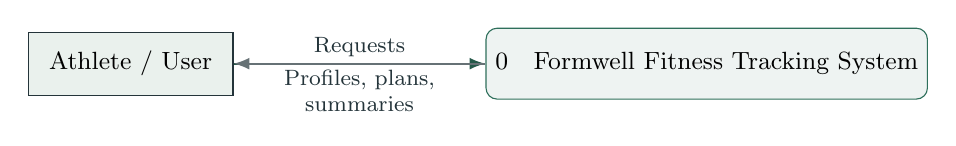
\begin{tikzpicture}[node distance=3.2cm]
\node[dfdentity] (user) {Athlete / User};
\node[process,right=of user,minimum width=4.6cm] (system) {0\quad Formwell Fitness Tracking System};
\draw[flow] (user) -- node[above,text width=2.4cm,align=center,flowlabel]{Requests} (system);
\draw[softflow] (system) -- node[below,text width=2.4cm,align=center,flowlabel]{Profiles, plans, summaries} (user);
\end{tikzpicture}}
\caption{Level-0 Context Data Flow Diagram (DFD).}
\label{fig:dfd0}
\end{figure}

The Level-1 DFD (Figure~\ref{fig:dfd1}) decomposes process 0 into authentication and profile management (1.0), plan retrieval (2.0), and daily activity logging and history review (3.0). The user symbol is repeated for layout clarity; each copy represents the same external entity. Every data store exchanges data through a process, with no direct store-to-store flows.

\begin{figure}[htbp]
\centering
\resizebox{\linewidth}{!}{
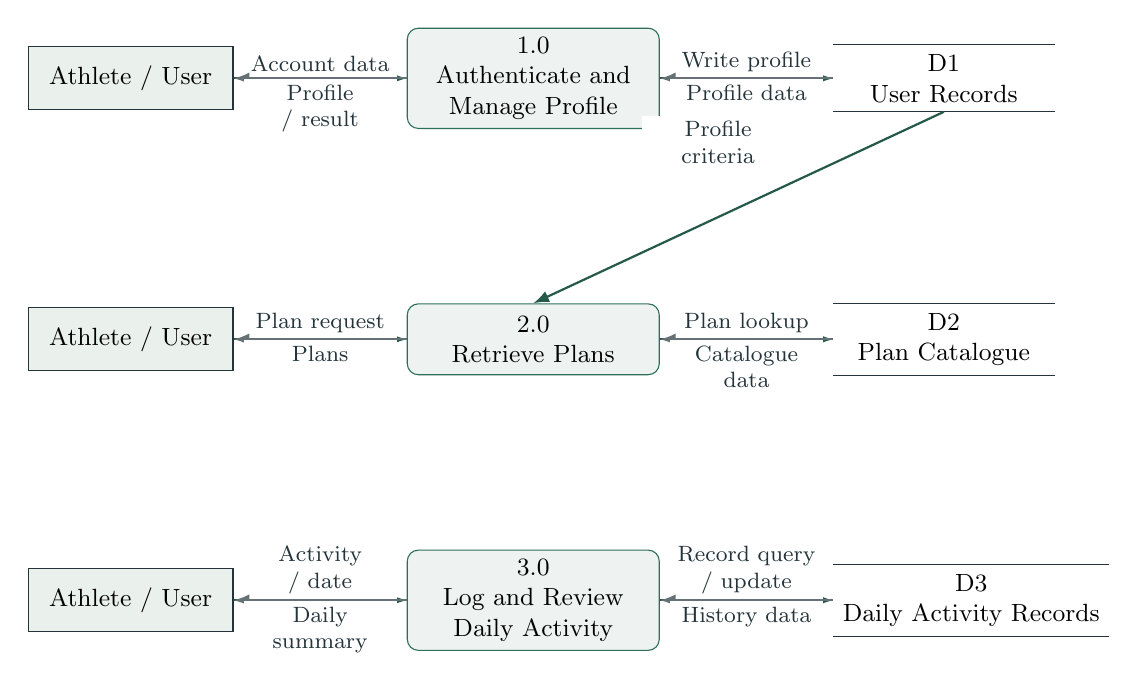
\begin{tikzpicture}[node distance=2.5cm and 2.2cm]
\node[dfdentity] (u1) {Athlete / User};
\node[process,right=of u1,minimum width=3.2cm] (auth) {1.0\\Authenticate and\\Manage Profile};
\node[store,right=of auth,minimum width=2.8cm] (users) {D1\\User Records};

\node[dfdentity,below=of u1] (u2) {Athlete / User};
\node[process,right=of u2,minimum width=3.2cm] (plan) {2.0\\Retrieve Plans};
\node[store,right=of plan,minimum width=2.8cm] (plans) {D2\\Plan Catalogue};

\node[dfdentity,below=of u2] (u3) {Athlete / User};
\node[process,right=of u3,minimum width=3.2cm] (log) {3.0\\Log and Review\\Daily Activity};
\node[store,right=of log,minimum width=2.8cm] (logs) {D3\\Daily Activity Records};

\draw[flow] (u1) -- node[above,text width=1.8cm,align=center,flowlabel]{Account data} (auth);
\draw[softflow] (auth) -- node[below,text width=1.8cm,align=center,flowlabel]{Profile / result} (u1);
\draw[flow] (auth) -- node[above,text width=1.8cm,align=center,flowlabel]{Write profile} (users);
\draw[softflow] (users) -- node[below,text width=1.8cm,align=center,flowlabel]{Profile data} (auth);
\draw[flow] (users.south) -- node[pos=0.55,above=6mm,text width=1.8cm,flowlabel]{Profile criteria} (plan.north);

\draw[flow] (u2) -- node[above,text width=1.8cm,align=center,flowlabel]{Plan request} (plan);
\draw[softflow] (plan) -- node[below,text width=1.8cm,align=center,flowlabel]{Plans} (u2);
\draw[flow] (plan) -- node[above,text width=1.8cm,align=center,flowlabel]{Plan lookup} (plans);
\draw[softflow] (plans) -- node[below,text width=1.8cm,align=center,flowlabel]{Catalogue data} (plan);

\draw[flow] (u3) -- node[above,text width=1.8cm,align=center,flowlabel]{Activity / date} (log);
\draw[softflow] (log) -- node[below,text width=1.8cm,align=center,flowlabel]{Daily summary} (u3);
\draw[flow] (log) -- node[above,text width=1.8cm,align=center,flowlabel]{Record query / update} (logs);
\draw[softflow] (logs) -- node[below,text width=1.8cm,align=center,flowlabel]{History data} (log);
\end{tikzpicture}}
\caption{Level-1 System Data Flow Diagram.}
\label{fig:dfd1}
\end{figure}

The following Level-2 DFDs decompose each Level-1 process. Each process exchanges data only with an external entity or a data store through a process; no external-entity-to-store or store-to-store flow is shown.

\begin{figure}[htbp]
\centering
\resizebox{0.92\linewidth}{!}{
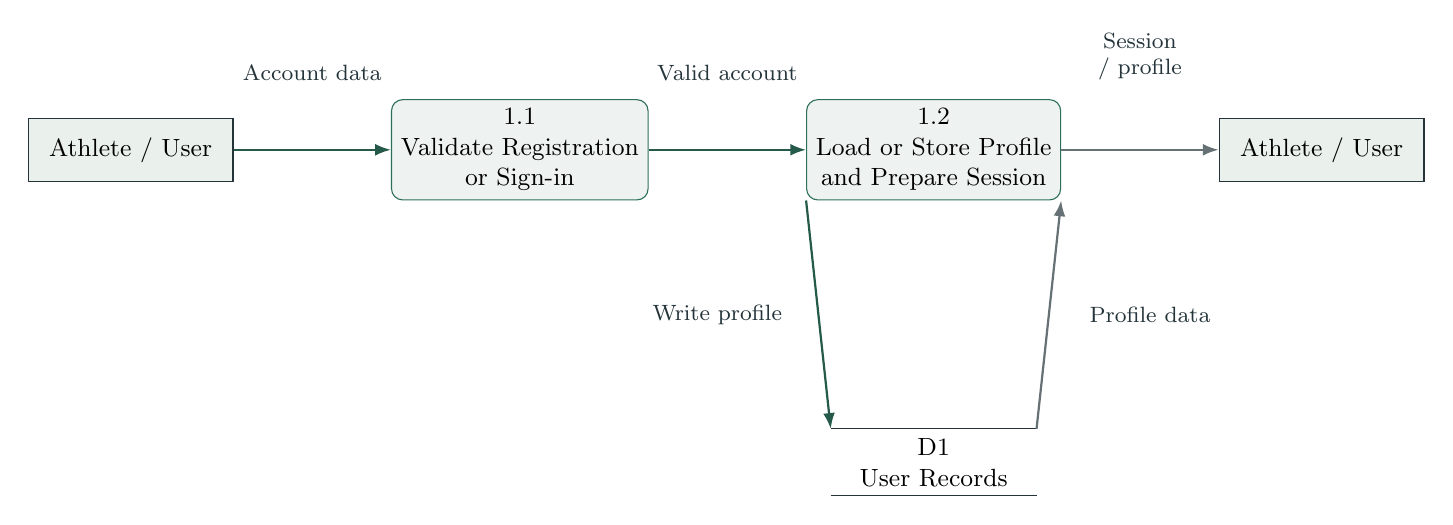
\begin{tikzpicture}[node distance=2.2cm and 2cm]
\node[dfdentity] (u) {Athlete / User};
\node[process,right=of u,minimum width=3.2cm] (verify) {1.1\\Validate Registration\\or Sign-in};
\node[process,right=of verify,minimum width=3.2cm] (profile) {1.2\\Load or Store Profile\\and Prepare Session};
\node[dfdentity,right=of profile] (userout) {Athlete / User};
\node[store,below=of profile,yshift=-0.7cm] (users) {D1\\User Records};

\draw[flow] (u) -- node[above=8mm,text width=1.8cm,align=center,flowlabel]{Account data} (verify);
\draw[flow] (verify) -- node[above=8mm,text width=1.8cm,align=center,flowlabel]{Valid account} (profile);
\draw[softflow] (profile) -- node[above=8mm,text width=1.8cm,align=center,flowlabel]{Session / profile} (userout);
\draw[flow] (profile.south west) -- node[left=3mm,text width=1.8cm,align=right,flowlabel]{Write profile} (users.north west);
\draw[softflow] (users.north east) -- node[right=3mm,text width=1.8cm,align=left,flowlabel]{Profile data} (profile.south east);
\end{tikzpicture}}
\caption{Level-2 DFD: Decomposition of Authentication and Profile Management (Process 1.0).}
\label{fig:dfd2_auth}
\end{figure}

\begin{figure}[htbp]
\centering
\resizebox{\linewidth}{!}{
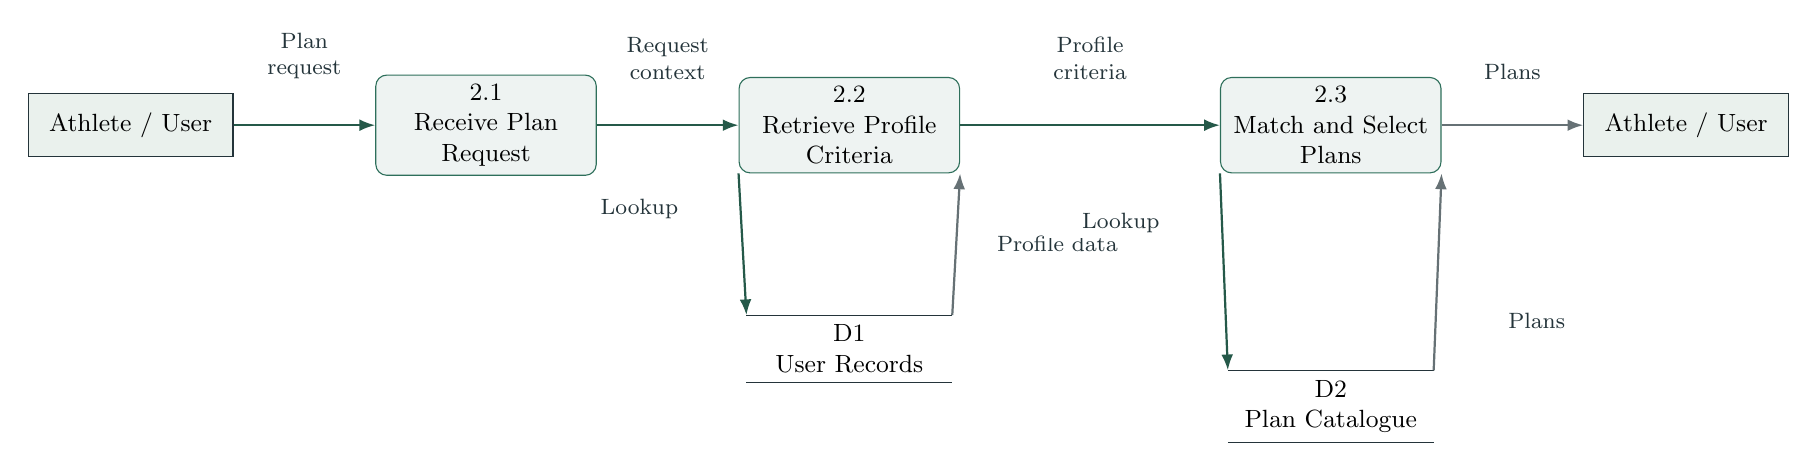
\begin{tikzpicture}[node distance=1.8cm and 1.8cm]
\node[dfdentity] (u) {Athlete / User};
\node[process,right=of u] (request) {2.1\\Receive Plan\\Request};
\node[process,right=of request] (profile) {2.2\\Retrieve Profile\\Criteria};
\node[process,right=of profile,xshift=1.5cm] (select) {2.3\\Match and Select\\Plans};
\node[store,below=of profile] (users) {D1\\User Records};
\node[store,below=of select,yshift=-0.7cm] (catalog) {D2\\Plan Catalogue};
\node[dfdentity,right=of select] (userout) {Athlete / User};

\draw[flow] (u) -- node[above=5mm,text width=1.4cm,align=center,flowlabel]{Plan request} (request);
\draw[flow] (request) -- node[above=5mm,text width=1.5cm,align=center,flowlabel]{Request context} (profile);
\draw[flow] (profile) -- node[above=5mm,text width=1.4cm,align=center,flowlabel]{Profile criteria} (select);
\draw[softflow] (select) -- node[above=5mm,text width=1.5cm,align=center,flowlabel]{Plans} (userout);
\draw[flow] (profile.south west) -- node[pos=0.25,left=3mm,text width=1.8cm,align=right,flowlabel]{Lookup} (users.north west);
\draw[softflow] (users.north east) -- node[right=3mm,text width=1.8cm,align=left,flowlabel]{Profile data} (profile.south east);
\draw[flow] (select.south west) -- node[pos=0.25,left=3mm,text width=1.8cm,align=right,flowlabel]{Lookup} (catalog.north west);
\draw[softflow] (catalog.north east) -- node[pos=0.25,right=3mm,text width=1.8cm,align=left,flowlabel]{Plans} (select.south east);
\end{tikzpicture}}
\caption{Level-2 DFD: Decomposition of Plan Retrieval (Process 2.0).}
\label{fig:dfd2_plan}
\end{figure}

\begin{figure}[htbp]
\centering
\resizebox{\linewidth}{!}{
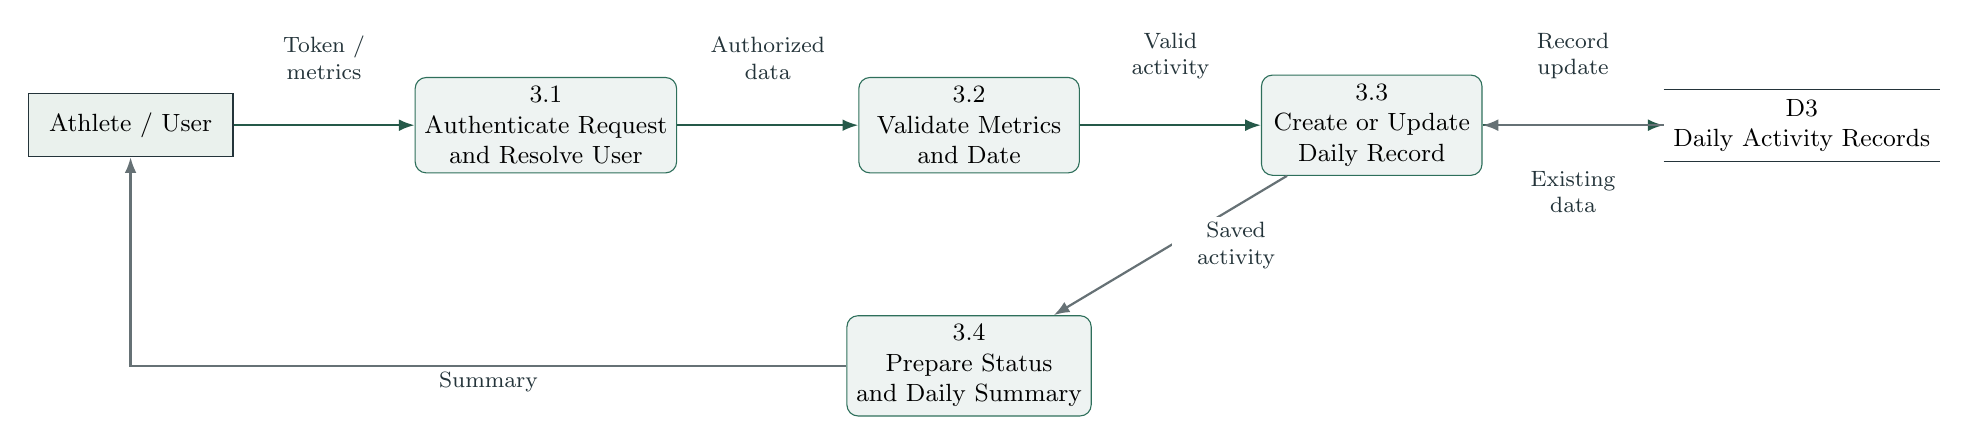
\begin{tikzpicture}[node distance=1.8cm and 2.3cm]
\node[dfdentity] (u) {Athlete / User};
\node[process,right=of u] (auth) {3.1\\Authenticate Request\\and Resolve User};
\node[process,right=of auth] (valid) {3.2\\Validate Metrics\\and Date};
\node[process,right=of valid] (upsert) {3.3\\Create or Update\\Daily Record};
\node[store,right=of upsert] (db) {D3\\Daily Activity Records};
\node[process,below=of valid] (response) {3.4\\Prepare Status\\and Daily Summary};

\draw[flow] (u) -- node[above=5mm,text width=1.6cm,align=center,flowlabel]{Token / metrics} (auth);
\draw[flow] (auth) -- node[above=5mm,text width=1.6cm,align=center,flowlabel]{Authorized data} (valid);
\draw[flow] (valid) -- node[above=5mm,text width=1.6cm,align=center,flowlabel]{Valid activity} (upsert);
\draw[flow] (upsert) -- node[above=5mm,text width=1.5cm,align=center,flowlabel]{Record update} (db);
\draw[softflow] (db) -- node[below=5mm,text width=1.5cm,align=center,flowlabel]{Existing data} (upsert);
\draw[softflow] (upsert) -- node[pos=0.5,right,text width=1.5cm,align=center,flowlabel]{Saved activity} (response);
\draw[softflow] (response.west) -| node[pos=0.25,below,text width=2cm,align=center,flowlabel]{Summary} (u.south);
\end{tikzpicture}}
\caption{Level-2 DFD: Decomposition of Daily Activity Logging and History Review (Process 3.0).}
\label{fig:dfd2_activity}
\end{figure}

\clearpage
\section{Proposed API Interface Specification}
The proposed browser-to-API interface uses JSON over HTTP during local development and HTTPS in deployment. Table~\ref{tab:routes} specifies resource-oriented routes and methods for the planned implementation.

\small
\begin{longtable}{P{0.38\linewidth}P{0.10\linewidth}P{0.16\linewidth}P{0.24\linewidth}}
\caption{Proposed RESTful HTTP API Route Inventory}\label{tab:routes}\\
\toprule
\textbf{Endpoint Path} & \textbf{Method} & \textbf{Protection} & \textbf{Functional Purpose} \\
\midrule
\endfirsthead
\toprule
\textbf{Endpoint Path} & \textbf{Method} & \textbf{Protection} & \textbf{Functional Purpose} \\
\midrule
\endhead
\url{/signup} & POST & Public & Register user profile and store hashed credentials. \\
\url{/login} & POST & Public & Verify credentials and issue signed JWT token. \\
\url{/check-auth} & GET & Bearer JWT & Validate active session token status. \\
\url{/users/me} & GET & Bearer JWT & Retrieve a sanitized profile baseline for the authenticated subject. \\
\url{/users/me/workout-plan} & GET & Bearer JWT & Retrieve the recommended strength training schedule. \\
\url{/users/me/cardio-plan} & GET & Bearer JWT & Retrieve the recommended cardio exercise schedule. \\
\url{/users/me/diet-plan} & GET & Bearer JWT & Retrieve the recommended weekday meal-plan content. \\
\url{/users/me/activity} & PUT & Bearer JWT & Create or update daily water, steps, and exercise counts. \\
\url{/users/me/activity/today} & GET & Bearer JWT & Retrieve current-day logged metrics and measurements. \\
\url{/users/me/activity/\{date\}} & GET & Bearer JWT & Retrieve historical metrics for an explicit calendar date. \\
\url{/users/me/targets/today} & GET & Bearer JWT & Retrieve current-day targets and completion values. \\
\url{/users/me/targets/\{date\}} & GET & Bearer JWT & Retrieve targets and completion values for the selected date. \\
\bottomrule
\end{longtable}

% -----------------------------------------------------------------------------
% Chapter 5: Analysis and Data Models
% -----------------------------------------------------------------------------
\chapter{Analysis and Data Models}

\section{Entity-Relationship Model}
The logical data model of Formwell is depicted in Figure~\ref{fig:er}. Solid connectors show database foreign-key relationships. Each workout mapping references exactly one body type, age group, cardio tier, and strength tier; each lookup row may be referenced by zero or more mappings. Daily logs belong to one user, and the unique constraint on (username, date) permits at most one log per user per date. Exercise targets reference an age group through a unique foreign key, so an age group has at most one target row. Schedule and diet tables are seeded catalogs selected by application code; they have no declared foreign keys to the tier tables and are therefore shown separately.

\begin{figure}[htbp]
\centering
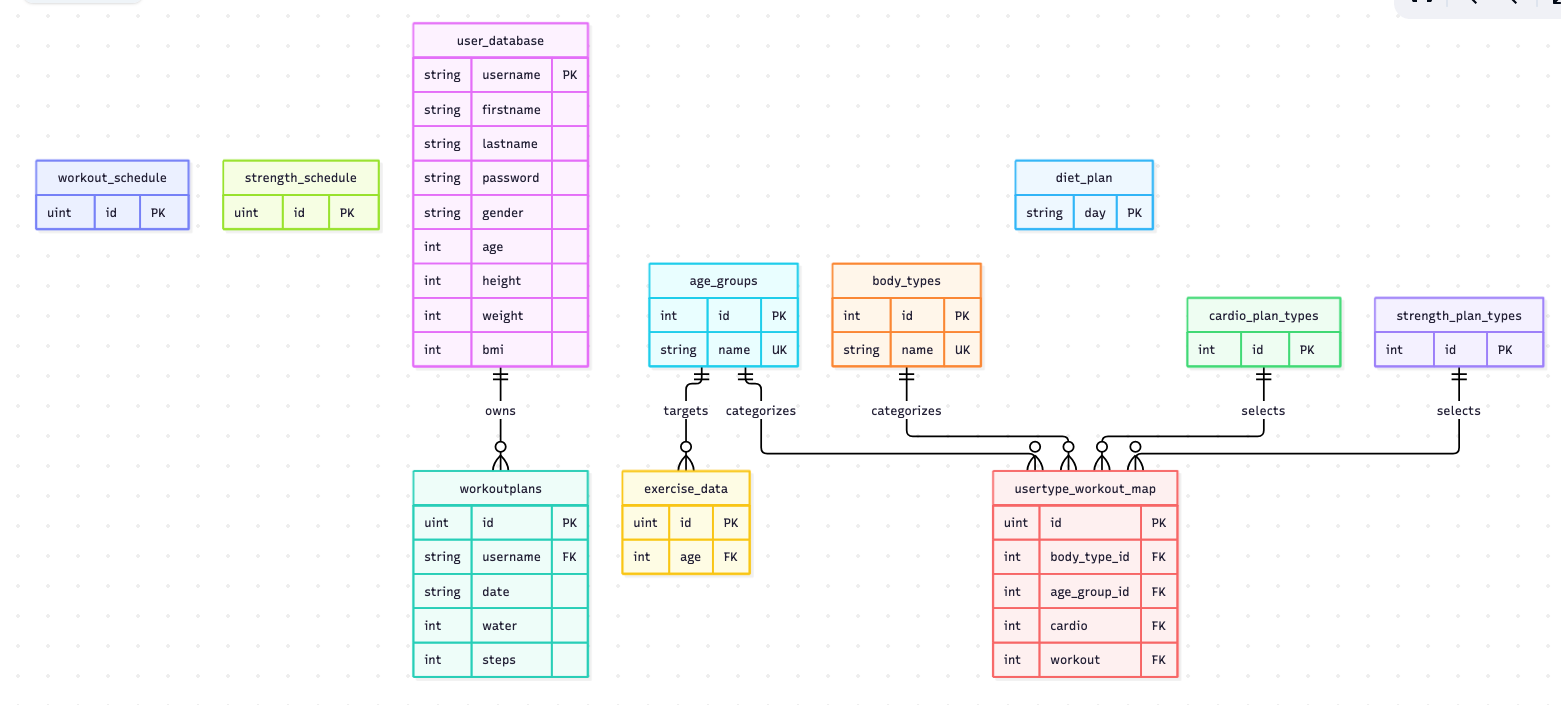
\includegraphics[width=\linewidth]{ER.png}
\caption{Proposed Entity-Relationship (ER) Diagram.}
\label{fig:er}
\end{figure}

\section{User Workflow and Activity Diagram}
Figure~\ref{fig:activity} uses UML activity notation. It shows session validation, the authenticated dashboard, guarded navigation choices, and the activity paths available to the user.

\begin{figure}[htbp]
\centering
\resizebox{0.94\linewidth}{!}{
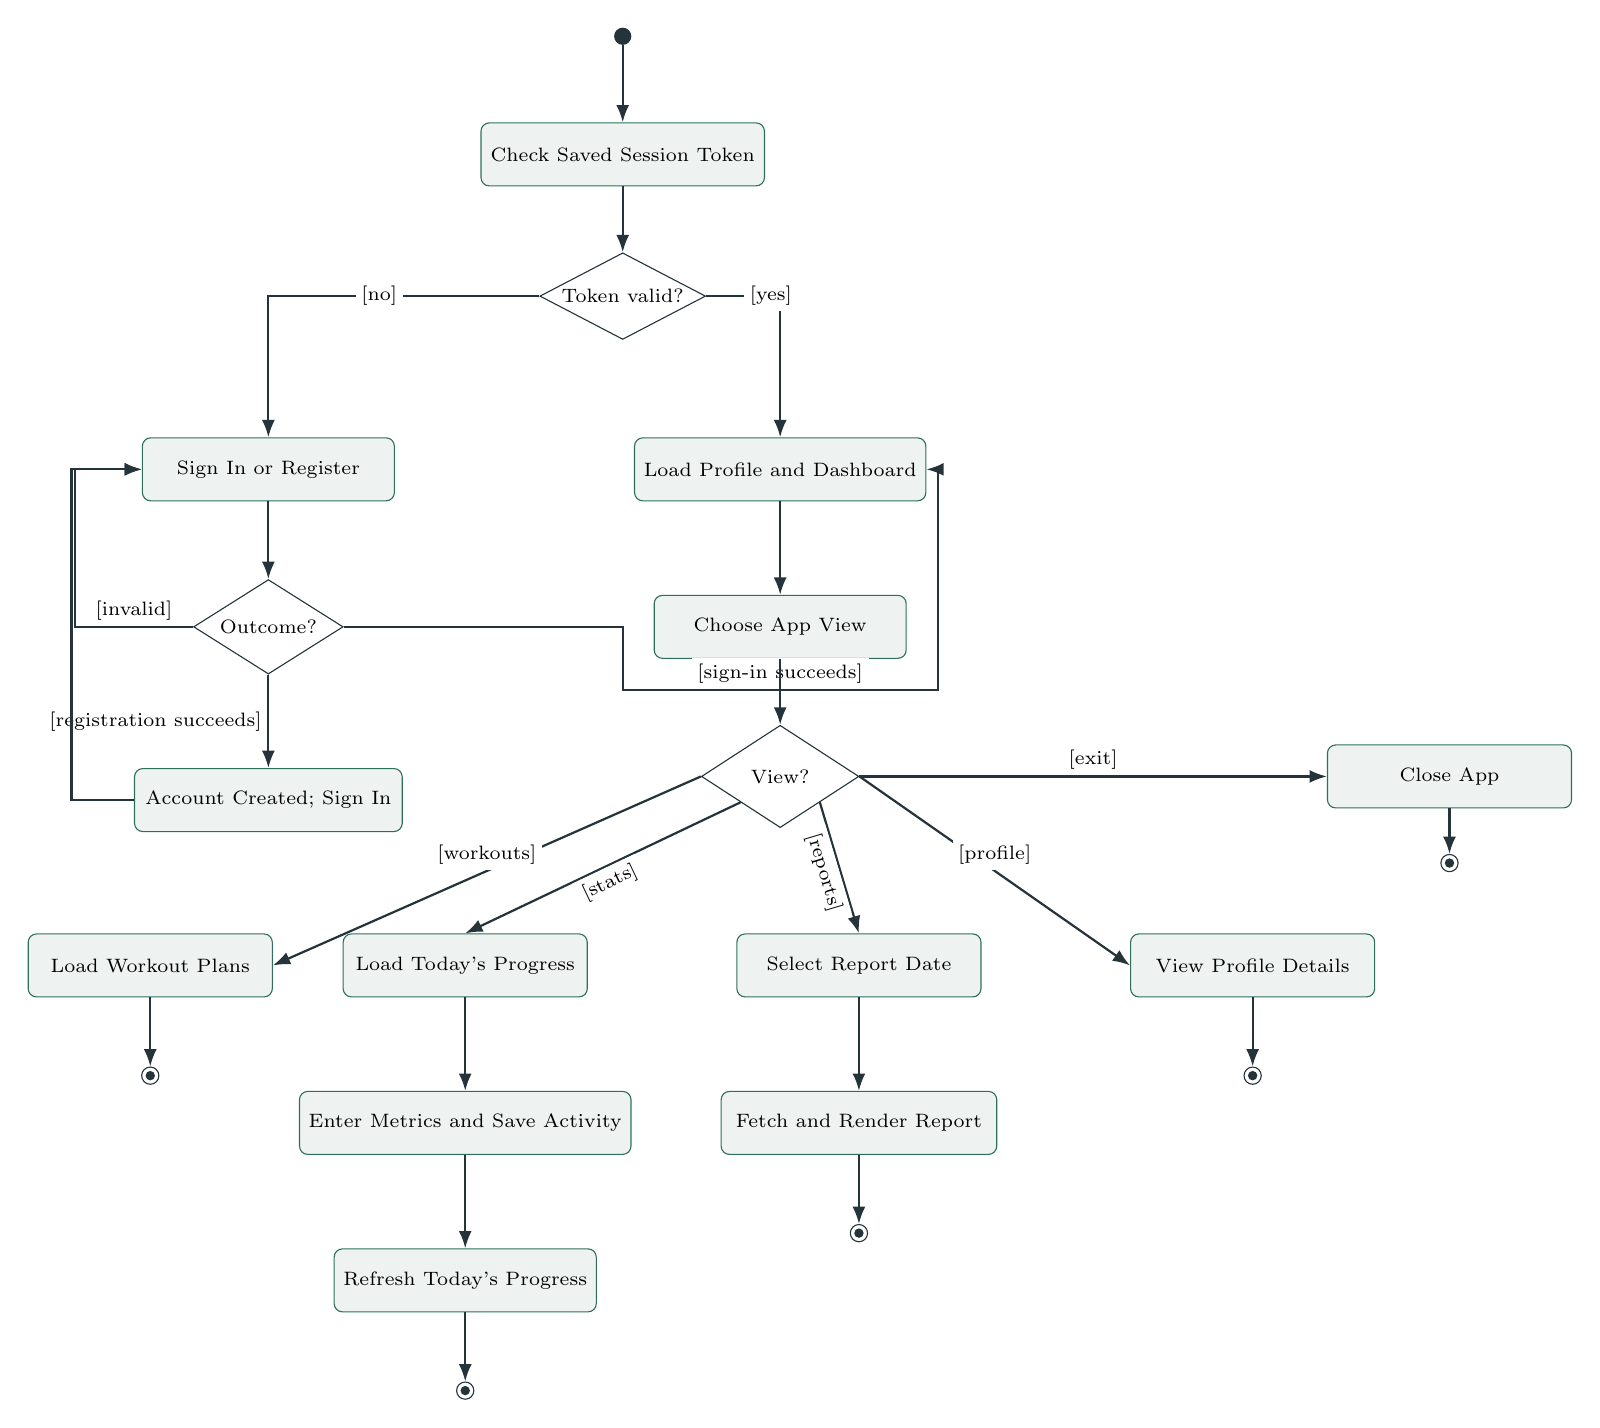
\begin{tikzpicture}[every node/.append style={font=\scriptsize}]
\node[circle,fill=ink,inner sep=2.2pt] (start) at (0,8) {};
\node[activityaction,minimum width=3.6cm] (session) at (0,6.5) {Check Saved Session Token};
\node[activitydecision,minimum width=1.7cm,minimum height=1.1cm] (valid) at (0,4.7) {Token valid?};
\node[activityaction] (auth) at (-4.5,2.5) {Sign In or Register};
\node[activitydecision,minimum width=1.9cm,minimum height=1.2cm] (signedin) at (-4.5,0.5) {Outcome?};
\node[activityaction,minimum width=3.4cm] (created) at (-4.5,-1.7) {Account Created; Sign In};
\node[activityaction,minimum width=3.6cm] (dashboard) at (2,2.5) {Load Profile and Dashboard};
\node[activityaction] (menu) at (2,0.5) {Choose App View};
\node[activitydecision,minimum width=2.0cm,minimum height=1.3cm] (choice) at (2,-1.4) {View?};

\node[activityaction,minimum width=3.1cm] (plans) at (-6,-3.8) {Load Workout Plans};
\node[activityaction,minimum width=3.1cm] (stats) at (-2,-3.8) {Load Today's Progress};
\node[activityaction,minimum width=3.5cm] (save) at (-2,-5.8) {Enter Metrics and Save Activity};
\node[activityaction,minimum width=3.1cm] (refresh) at (-2,-7.8) {Refresh Today's Progress};
\node[activityaction,minimum width=3.1cm] (reports) at (3,-3.8) {Select Report Date};
\node[activityaction,minimum width=3.5cm] (report) at (3,-5.8) {Fetch and Render Report};
\node[activityaction,minimum width=3.1cm] (profile) at (8,-3.8) {View Profile Details};
\node[activityaction,minimum width=3.1cm] (close) at (10.5,-1.4) {Close App};

\node[circle,draw=ink,fill=white,inner sep=2.2pt] (endplans) at (-6,-5.2) {};
\node[circle,fill=ink,inner sep=1.2pt] at (endplans) {};
\node[circle,draw=ink,fill=white,inner sep=2.2pt] (endstats) at (-2,-9.2) {};
\node[circle,fill=ink,inner sep=1.2pt] at (endstats) {};
\node[circle,draw=ink,fill=white,inner sep=2.2pt] (endreport) at (3,-7.2) {};
\node[circle,fill=ink,inner sep=1.2pt] at (endreport) {};
\node[circle,draw=ink,fill=white,inner sep=2.2pt] (endprofile) at (8,-5.2) {};
\node[circle,fill=ink,inner sep=1.2pt] at (endprofile) {};
\node[circle,draw=ink,fill=white,inner sep=2.2pt] (endclose) at (10.5,-2.5) {};
\node[circle,fill=ink,inner sep=1.2pt] at (endclose) {};

\draw[relation] (start) -- (session);
\draw[relation] (session) -- (valid);
\draw[relation] (valid.west) -| node[pos=.25,left,fill=white,inner sep=2pt]{[no]} (auth.north);
\draw[relation] (valid.east) -| node[pos=.25,right,fill=white,inner sep=2pt]{[yes]} (dashboard.north);
\draw[relation] (auth) -- (signedin);
\draw[relation] (signedin.west) -- node[above,fill=white,inner sep=2pt]{[invalid]} ++(-1.5,0) |- (auth.west);
\draw[relation] (signedin.east) -- (0,0.5) -- (0,-0.3) -- node[above,fill=white,inner sep=2pt]{[sign-in succeeds]} (4,-0.3) -- (4,2.5) -- (dashboard.east);
\draw[relation] (signedin.south) -- node[left,fill=white,inner sep=2pt]{[registration succeeds]} (created.north);
\draw[relation] (created.west) -- (-7,-1.7) |- (auth.west);
\draw[relation] (dashboard) -- (menu);
\draw[relation] (menu) -- (choice);
\draw[relation] (choice.west) -- node[above,fill=white,inner sep=2pt]{[workouts]} (plans.east);
\draw[relation] (choice.south west) -- node[below,sloped,fill=white,inner sep=2pt]{[stats]} (stats.north);
\draw[relation] (choice.south east) -- node[below,sloped,fill=white,inner sep=2pt]{[reports]} (reports.north);
\draw[relation] (choice.east) -- node[above,fill=white,inner sep=2pt]{[profile]} (profile.west);
\draw[relation] (choice.east) -- node[above,fill=white,inner sep=2pt]{[exit]} (close.west);
\draw[relation] (plans) -- (endplans);
\draw[relation] (stats) -- (save);
\draw[relation] (save) -- (refresh);
\draw[relation] (refresh) -- (endstats);
\draw[relation] (reports) -- (report);
\draw[relation] (report) -- (endreport);
\draw[relation] (profile) -- (endprofile);
\draw[relation] (close) -- (endclose);
\end{tikzpicture}}
\caption{UML Activity Diagram of the User Workflow.}
\label{fig:activity}
\end{figure}

% \section{Class and Component Architecture}
% Figure~\ref{fig:class} models the modular software component architecture, separating client-side presentation, HTTP routing, business services, GORM ORM data mapping, and PostgreSQL persistence.

% \begin{figure}[htbp]
% \centering
% \resizebox{\linewidth}{!}{
% \begin{tikzpicture}[node distance=0.65cm and 0.55cm]
% \node[entity] (frontend) {Client Browser UI\\HTML5 / CSS3 / JavaScript};
% \node[process,right=of frontend] (handlers) {Go HTTP Handlers\\\& JWT Middleware};
% \node[process,right=of handlers] (interface) {Database Service\\Repository Interface};
% \node[process,right=of interface] (mydb) {GORM Database\\Implementation};
% \node[store,right=of mydb] (pg) {PostgreSQL 16\\Database};
% \draw[relation] (frontend) -- node[above,font=\scriptsize]{JSON / HTTP} (handlers);
% \draw[relation] (handlers) -- node[above,font=\scriptsize]{Method Call} (interface);
% \draw[relation] (interface) -- node[above,font=\scriptsize]{GORM API} (mydb);
% \draw[relation] (mydb) -- node[above,font=\scriptsize]{SQL Queries} (pg);
% \end{tikzpicture}}
% \caption{Proposed Class and Component Architecture.}
% \label{fig:class}
% \end{figure}

\clearpage
\section{UML State Machine Model}
Figure~\ref{fig:state} uses UML state-machine notation to show the lifecycle of a daily activity submission. Guarded transitions distinguish malformed input, a missing or existing daily record, and successful or failed writes.

\begin{figure}[htbp]
\centering
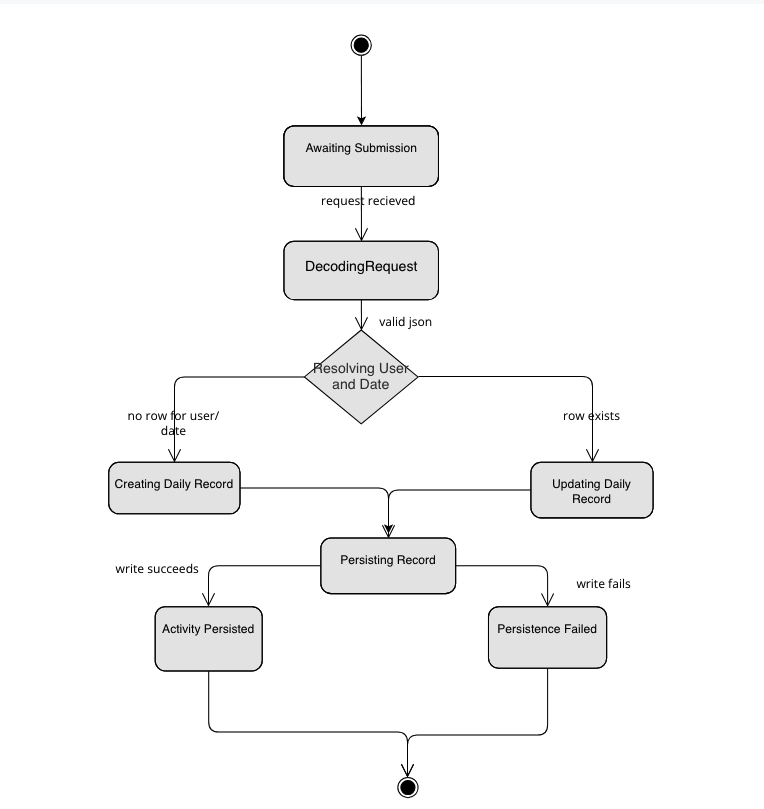
\includegraphics[width=0.9\linewidth]{statemachine.png}
\caption{UML State Machine for Daily Activity Submission.}
\label{fig:state}
\end{figure}

% -----------------------------------------------------------------------------
% Chapter 6: Database Design and Schema Specification
% -----------------------------------------------------------------------------
\chapter{Database Design and Schema Specification}\label{ch:database}

\section{Database Design Principles}
The proposed database separates user profiles, category lookups, category mappings, schedule catalogues, and user-day activity records. Primary and foreign keys and a composite unique key on user and date will protect core relationships. The schedule catalogues retain separate category-specific tables to reflect the project design; their duplication will be reviewed during schema refinement. The design will use suitable keys and constraints to protect data integrity. User and activity records will include creation and update timestamps; security events may be recorded without credentials or bearer tokens, subject to a retention policy.

\section{Core User and Daily Activity Schema}
Table~\ref{tab:core-schema} specifies the core relational schema for user authentication profiles and daily workout tracking.

\begin{longtable}{P{0.25\linewidth}P{0.68\linewidth}}
\caption{Core User and Daily Activity Relational Schema}\label{tab:core-schema}\\
\toprule
\textbf{Table Name / Key} & \textbf{Columns, Data Types, and Constraints} \\
\midrule
\endfirsthead
\toprule
\textbf{Table Name / Key} & \textbf{Columns, Data Types, and Constraints} \\
\midrule
\endhead
\texttt{user\_database} \newline \textbf{PK:} \texttt{username} & \texttt{username}: VARCHAR(64) PRIMARY KEY, NOT NULL; \newline \texttt{firstname}, \texttt{lastname}: VARCHAR(64), NOT NULL; \newline \texttt{password}: VARCHAR(255), NOT NULL (stores adaptive bcrypt hash); \newline \texttt{gender}: VARCHAR(16), NOT NULL; \newline \texttt{age}: INT, NOT NULL, CHECK (age $> 0$); \newline \texttt{height}: INT, NOT NULL, CHECK (height $> 0$); \newline \texttt{weight}: INT, NOT NULL, CHECK (weight $> 0$); \newline \texttt{bmi}: DECIMAL(5,2), NOT NULL, derived from height and weight; category boundaries shall be applied to the unrounded value. \\
\midrule
\texttt{workoutplans} \newline \textbf{PK:} \texttt{id} \newline \textbf{FK:} \texttt{username} & \texttt{id}: BIGSERIAL PRIMARY KEY; \newline \texttt{username}: VARCHAR(64) NOT NULL, FK references \texttt{user\_database(username)} ON UPDATE CASCADE ON DELETE CASCADE; \newline \texttt{date}: DATE NOT NULL; \newline \textbf{Composite Unique Index:} \texttt{idx\_user\_date} on (\texttt{username}, \texttt{date}). \\
\midrule
\texttt{workoutplans} \newline (Daily Metrics \& Exercise Counts) & Integer Daily Metrics: \texttt{water} (ml, non-negative), \texttt{steps} (count, non-negative). \newline Exercise Repetition Counts: \texttt{squatsdone}, \texttt{deadliftdone}, \texttt{pushupsdone}, \texttt{pullupsdone}, \texttt{jumpingjacksdone}, \texttt{weightliftdone}, \texttt{benchpressdone}, \texttt{lungesdone}, \texttt{legpressdone}, \texttt{runningdone}, \texttt{cyclingdone}, \texttt{swimmingdone}, \texttt{walkingdone} (all INT, default 0, CHECK $\ge 0$). \newline Each record shall also include \texttt{created\_at} and \texttt{updated\_at} timestamps. \\
\midrule
\texttt{workoutplans} \newline (Target Columns) & Target Baseline Columns: \texttt{squats}, \texttt{deadlift}, \texttt{pushups}, \texttt{pullups}, \texttt{jumpingjacks}, \texttt{weightlift}, \texttt{benchpress}, \texttt{lunges}, \texttt{legpress}, \texttt{running}, \texttt{cycling}, \texttt{swimming}, \texttt{walking} (VARCHAR(32), recommended baseline goals). \\
\bottomrule
\end{longtable}

\section{Category Lookup and Mapping Tables}
To support deterministic recommendation, the system employs lookup and mapping tables as detailed in Table~\ref{tab:lookup-schema}.

\begin{longtable}{P{0.25\linewidth}P{0.68\linewidth}}
\caption{Lookup and Recommendation Mapping Tables}\label{tab:lookup-schema}\\
\toprule
\textbf{Table Name} & \textbf{Columns, Data Types, and Constraints} \\
\midrule
\endfirsthead
\toprule
\textbf{Table Name} & \textbf{Columns, Data Types, and Constraints} \\
\midrule
\endhead
\texttt{body\_types} & \texttt{id}: INT PRIMARY KEY; \texttt{name}: VARCHAR(32) NOT NULL, UNIQUE. Seeded as rule-based BMI bands: \texttt{type\_1} below 18.5, \texttt{type\_2} from 18.5 to below 25, and \texttt{type\_3} at or above 25; these are selectors for catalogue content, not clinical assessments. \\
\texttt{age\_groups} & \texttt{id}: INT PRIMARY KEY; \texttt{name}: VARCHAR(32) NOT NULL, UNIQUE. Seeded with age tiers (\texttt{group\_1}: below 20; \texttt{group\_2}: 20--40 inclusive; \texttt{group\_3}: above 40). \\
\texttt{cardio\_plan\_types} & \texttt{id}: INT PRIMARY KEY. Seeded identifiers 1--3 corresponding to cardio schedule tiers. \\
\texttt{strength\_plan\_types} & \texttt{id}: INT PRIMARY KEY. Seeded identifiers 1--3 corresponding to strength schedule tiers. \\
\texttt{usertype\_workout\_map} & \texttt{id}: BIGSERIAL PRIMARY KEY; \texttt{body\_type\_id}, \texttt{age\_group\_id}, \texttt{cardio}, \texttt{workout}: INT NOT NULL; \newline \textbf{Composite Unique Index:} on (\texttt{body\_type\_id}, \texttt{age\_group\_id}); \newline FKs referencing lookup tables with ON UPDATE CASCADE ON DELETE RESTRICT. \\
\texttt{exercise\_data} & \texttt{id}: BIGSERIAL PRIMARY KEY; \texttt{age}: INT NOT NULL UNIQUE, FK to \texttt{age\_groups(id)}; thirteen target fields defining baseline daily goals for each age bracket. \\
\bottomrule
\end{longtable}

\section{Workout and Diet Schedule Catalogues}
The proposed database will store the schedule catalogues in category-specific relations, with a schema review to consolidate shared fields where practical:
\begin{itemize}
  \item \textbf{Cardio Schedules (\texttt{workout\_schedule1--3}):} Contain structured routines for each day of the week (\texttt{monday} through \texttt{sunday}, VARCHAR(255) NOT NULL).
  \item \textbf{Strength Schedules (\texttt{strength\_schedule1--3}):} Detail specific muscle group splits and exercises for all seven calendar days.
  \item \textbf{Dietary Plans (\texttt{diet\_plan1--3}):} Map days of the week (\texttt{day}: PK) to balanced nutritional recommendations covering \texttt{breakfast}, \texttt{lunch}, and \texttt{dinner}.
\end{itemize}

% -----------------------------------------------------------------------------
% Chapter 7: Modular Structure and Implementation Methodology
% -----------------------------------------------------------------------------
\chapter{Modular Structure and Implementation Methodology}

\section{Module Decomposition and Planned Effort}
The proposed system is decomposed into nine functional modules (M1--M9). The illustrative effort estimate is 36 person-days across the planned eight-week lifecycle, as shown in Table~\ref{tab:modules}; it will be reviewed with the project guide.

\begin{table}[htbp]
\centering
\caption{Proposed System Modules and Development Allocation}
\label{tab:modules}
\begin{tabularx}{\linewidth}{P{0.08\linewidth}P{0.24\linewidth}Y P{0.1\linewidth}P{0.14\linewidth}}
\toprule
\textbf{ID} & \textbf{Module Name} & \textbf{Core Functional Responsibility} & \textbf{Effort} & \textbf{Phase} \\
\midrule
M1 & Identity \& Session & User signup, bcrypt password hashing, login verification, JWT token issuance, and logout session clearing. & 4 days & Phase 2 \\
M2 & Profile \& Baseline & Height/weight ingestion, automated BMI calculation, physical baseline storage, and profile dashboard rendering. & 3 days & Phase 2 \\
M3 & Plan Catalog Engine & Biometric classification, age/BMI mapping algorithm, and retrieval of curated cardio, strength, and diet schedules. & 5 days & Phase 2 \\
M4 & Daily Activity Ingestion & Forms for water, steps, and 13 exercise counts; input sanitization; atomic upsert under user/date unique key. & 4 days & Phase 3 \\
M5 & Progress Analytics & Date-picker query engine, historical record retrieval, progress calculation against target baselines, and report rendering. & 3 days & Phase 3 \\
M6 & Core REST API & Go ServeMux routing, CORS policy middleware, JSON request decoding, and GORM database repository interface. & 5 days & Phase 2 \\
M7 & Responsive UI & Modular HTML5 templates, fluid CSS3 Grid/Flexbox styling, client-side validation, and asynchronous fetch handlers. & 5 days & Phase 3 \\
M8 & Security \& Testing & Subject-to-token authorization checks, unit tests, integration testing, and vulnerability remediation. & 5 days & Phase 4 \\
M9 & DevOps \& Packaging & Dockerfile multi-stage builds, Docker Compose configuration, automated database seeding, and final documentation. & 2 days & Phase 5 \\
\midrule
\multicolumn{3}{r}{\textbf{Total Estimated Development Effort:}} & \textbf{36 days} & \\
\bottomrule
\end{tabularx}
\end{table}

\section{Process Logic and Core Algorithms}
The proposed system will use three deterministic processes:
\begin{enumerate}
  \item \textbf{BMI Derivation and Rule-Based Category Assignment:}
  \begin{equation}
    \text{BMI} = \frac{\text{weight (kg)}}{(\text{height (m)})^2} = \frac{\text{weight (kg)} \times 10{,}000}{(\text{height (cm)})^2}
  \end{equation}
  For the project catalogue, the derived BMI will be assigned to these rule-based tiers (not medical diagnoses): lower BMI band ($\text{BMI} < 18.5$, \texttt{type\_1}), middle BMI band ($18.5 \le \text{BMI} < 25.0$, \texttt{type\_2}), and upper BMI band ($\text{BMI} \ge 25.0$, \texttt{type\_3}).
  \item \textbf{Deterministic Routine Mapping Algorithm:} Given the authenticated user's body type $B \in \{1, 2, 3\}$ and age group $A \in \{1, 2, 3\}$, the system queries the associative relation:
  \begin{equation}
    (B, A) \xrightarrow{\text{usertype\_workout\_map}} (\text{CardioTier}, \text{StrengthTier})
  \end{equation}
  The resolved tier identifiers determine the exact schedule and diet catalogs delivered to the client.
  \item \textbf{Idempotent Daily Logging Algorithm:} When a daily log payload is received for user $U$ and calendar date $D$, the system queries \texttt{workoutplans} for the tuple $(U, D)$. The API will use the composite unique key and a transactional upsert to prevent duplicate records. The record will include or reference the applicable target values from \texttt{exercise\_data}.
\end{enumerate}

% \section{Audit and Data Lifecycle Design}
% The proposed records will carry creation and update timestamps. Authentication failures and application errors may be recorded as operational events, but passwords, password hashes, and bearer tokens shall not be written to logs. A retention and account-deletion policy will be defined before any deployment involving real user data.

\section{Core Data Structures}
Table~\ref{tab:structures} outlines the primary data structures across the application layers.

\begin{table}[htbp]
\centering
\caption{Principal Data Structures Across Application Layers}
\label{tab:structures}
\begin{tabularx}{\linewidth}{P{0.22\linewidth}P{0.25\linewidth}Y}
\toprule
\textbf{System Layer} & \textbf{Data Structure} & \textbf{Purpose and Application} \\
\midrule
Browser Client & Plain JavaScript Objects & Dynamic form state, cached profile attributes, and asynchronous JSON payloads. \\
Browser State & In-memory session state & Short-lived access token and active profile data; persistent browser storage of bearer tokens will be avoided. \\
API Layer & Go Structs (\texttt{User}, \texttt{Workoutplan}) & Strongly typed domain models with JSON and GORM struct tags. \\
API Context & JWT Claims Struct & Contextual user claims (\texttt{Username}, \texttt{ExpiresAt}) carried within authenticated request contexts. \\
Persistence Layer & PostgreSQL Relations & ACID-compliant relational tables enforcing constraints and indexing. \\
\bottomrule
\end{tabularx}
\end{table}

% -----------------------------------------------------------------------------
% Chapter 8: Project Planning, Scheduling, and Risk Management
% -----------------------------------------------------------------------------
\chapter{Project Planning, Scheduling, and Risk Management}

\section{Methodology and Phased Execution}
The project will be executed using an iterative, phased software development lifecycle organized into five distinct phases over eight calendar weeks:
\begin{itemize}
  \item \textbf{Phase 1: Inception \& Architectural Specification (Weeks 1--2):} Requirements finalization, database normalization, API contract definition, and project approval.
  \item \textbf{Phase 2: Core Backend \& Persistence Development (Weeks 2--4):} Go HTTP API scaffolding, PostgreSQL GORM integration, bcrypt authentication, and plan engine.
  \item \textbf{Phase 3: Frontend Implementation \& Integration (Weeks 3--6):} Responsive UI views, asynchronous client request helpers, daily logging forms, and dashboard analytics.
  \item \textbf{Phase 4: Security Hardening \& Quality Assurance (Weeks 6--7):} Subject authorization enforcement, comprehensive unit and API integration testing, and bug remediation.
  \item \textbf{Phase 5: Packaging, Deployment \& Evaluation (Weeks 7--8):} Docker containerization, final user acceptance testing, and academic project report preparation.
\end{itemize}

\section{Proposed Gantt Schedule}
Figure~\ref{fig:gantt} illustrates the planned timeline and task overlaps across the eight-week execution window.

\begin{figure}[htbp]
\centering
\resizebox{\linewidth}{!}{
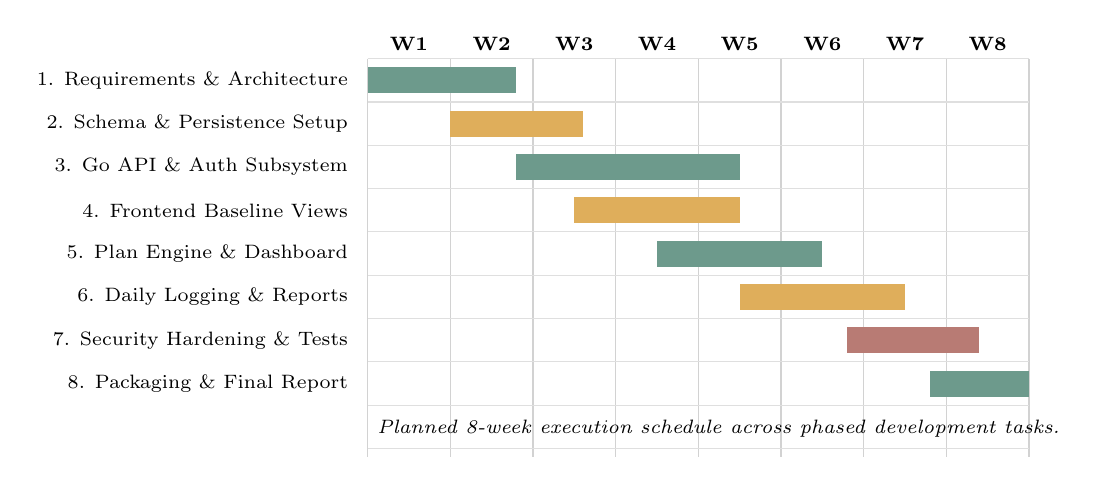
\begin{tikzpicture}[x=1.05cm,y=0.55cm]
\foreach \x in {0,...,8} {\draw[gray!35] (\x,0) -- (\x,-9.2);}
\foreach \y in {0,...,9} {\draw[gray!25] (0,-\y) -- (8,-\y);}
\foreach \x in {1,...,8} {\node[font=\scriptsize\bfseries] at (\x-0.5,0.35) {W\x};}
\node[anchor=east,font=\scriptsize,align=right] at (-0.12,-0.5) {1. Requirements \& Architecture};
\node[anchor=east,font=\scriptsize,align=right] at (-0.12,-1.5) {2. Schema \& Persistence Setup};
\node[anchor=east,font=\scriptsize,align=right] at (-0.12,-2.5) {3. Go API \& Auth Subsystem};
\node[anchor=east,font=\scriptsize,align=right] at (-0.12,-3.5) {4. Frontend Baseline Views};
\node[anchor=east,font=\scriptsize,align=right] at (-0.12,-4.5) {5. Plan Engine \& Dashboard};
\node[anchor=east,font=\scriptsize,align=right] at (-0.12,-5.5) {6. Daily Logging \& Reports};
\node[anchor=east,font=\scriptsize,align=right] at (-0.12,-6.5) {7. Security Hardening \& Tests};
\node[anchor=east,font=\scriptsize,align=right] at (-0.12,-7.5) {8. Packaging \& Final Report};
\fill[green!70] (0,-0.8) rectangle (1.8,-0.2);
\fill[gold!80] (1.0,-1.8) rectangle (2.6,-1.2);
\fill[green!70] (1.8,-2.8) rectangle (4.5,-2.2);
\fill[gold!80] (2.5,-3.8) rectangle (4.5,-3.2);
\fill[green!70] (3.5,-4.8) rectangle (5.5,-4.2);
\fill[gold!80] (4.5,-5.8) rectangle (6.5,-5.2);
\fill[red!70] (5.8,-6.8) rectangle (7.4,-6.2);
\fill[green!70] (6.8,-7.8) rectangle (8.0,-7.2);
\node[anchor=west,font=\scriptsize\itshape] at (0,-8.55) {Planned 8-week execution schedule across phased development tasks.};
\end{tikzpicture}}
\caption{Proposed Eight-Week Project Gantt Schedule.}
\label{fig:gantt}
\end{figure}

\section{PERT Precedence Network and Critical Path}
Figure~\ref{fig:pert} models the task dependencies and precedence constraints. The critical path spans activities A $\rightarrow$ B $\rightarrow$ C $\rightarrow$ D $\rightarrow$ E $\rightarrow$ F $\rightarrow$ G $\rightarrow$ H, totaling 38 sequential working days. At five working days per week, this is approximately eight work weeks; the Gantt schedule uses limited task overlap and remains subject to the academic calendar.

\begin{figure}[htbp]
\centering
\resizebox{0.94\linewidth}{!}{
\begin{tikzpicture}[node distance=1.15cm and 1.25cm]
\node[process] (a) {A\ Requirements\\3 days};
\node[process,right=of a] (b) {B\ Schema Design\\5 days};
\node[process,right=of b] (c) {C\ API Core\\9 days};
\node[process,right=of c] (d) {D\ Frontend\\8 days};
\node[process,right=of d] (e) {E\ Integration\\4 days};
\node[process,right=of e] (f) {F\ Security \& Tests\\5 days};
\node[process,right=of f] (g) {G\ Verification\\2 days};
\node[process,right=of g] (h) {H\ Final Report\\2 days};
\draw[relation] (a) -- (b);
\draw[relation] (b) -- (c);
\draw[relation] (c) -- (d);
\draw[relation] (d) -- (e);
\draw[relation] (e) -- (f);
\draw[relation] (f) -- (g);
\draw[relation] (g) -- (h);
\end{tikzpicture}}
\caption{Proposed Project PERT Precedence Network.}
\label{fig:pert}
\end{figure}

% \section{Risk Assessment and Mitigation Strategies}
% Table~\ref{tab:risks} identifies anticipated technical risks and establishes proactive mitigation measures.

% \begin{table}[htbp]
% \centering
% \caption{Project Technical Risks and Proactive Engineering Mitigations}
% \label{tab:risks}
% \begin{tabularx}{\linewidth}{P{0.24\linewidth}P{0.28\linewidth}Y}
% \toprule
% \textbf{Identified Technical Risk} & \textbf{Potential Impact} & \textbf{Proactive Mitigation Strategy} \\
% \midrule
% Plaintext credential exposure & Unauthorized credential compromise and database breach vulnerability. & Implement bcrypt hashing with a benchmarked work factor of at least 10; use dedicated response DTOs that omit password fields. \\
% Cross-account authorization bypass & Unauthorized users reading or modifying other users' profiles/logs. & Enforce token-bound subject extraction; verify that path identifiers strictly match authenticated token claims. \\
% Midnight calendar boundary drift & Metrics recorded under incorrect calendar date when session spans midnight. & Standardize date generation at request time using explicit ISO-8601 UTC date parsing in business logic. \\
% Unsanitized input injection & Malformed payloads causing SQL errors or database corruption. & Implement strict server-side JSON schema validation, non-negative bounds checks, and parameterized GORM queries. \\
% Schema migration regressions & Loss of referential integrity or broken table states during iterations. & Maintain structured, repeatable database migration scripts and automated Docker seeding fixtures. \\
% \bottomrule
% \end{tabularx}
% \end{table}

% -----------------------------------------------------------------------------
% Chapter 9: Network Architecture and Security Design
% -----------------------------------------------------------------------------
\chapter{Network Architecture and Security Design}

\section{Proposed Network Deployment Topology}
Figure~\ref{fig:network} models the network topology and trust boundaries. The frontend will communicate with the Go API over HTTP during isolated local development and HTTPS in deployment. The API and PostgreSQL will communicate over a private service network. TLS will be configured for production connections where supported by the hosting environment.

\begin{figure}[htbp]
\centering
\resizebox{0.92\linewidth}{!}{
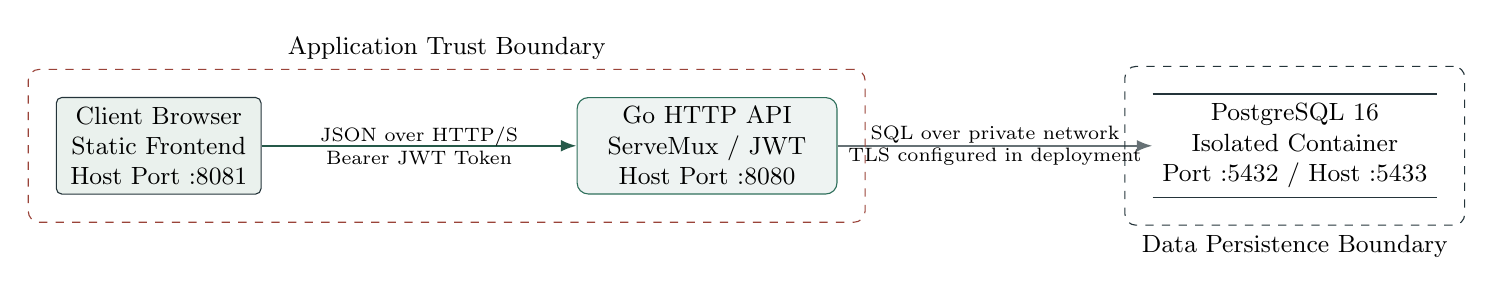
\begin{tikzpicture}[node distance=1.8cm and 4cm]
\node[entity] (browser) {Client Browser\\Static Frontend\\Host Port :8081};
\node[process,right=of browser,minimum width=3.3cm] (api) {Go HTTP API\\ServeMux / JWT\\Host Port :8080};
\node[store,right=of api,minimum width=3.2cm] (pg) {PostgreSQL 16\\Isolated Container\\Port :5432 / Host :5433};
\draw[flow] (browser) -- node[midway,align=center,font=\scriptsize]{JSON over HTTP/S\\Bearer JWT Token} (api);
\draw[softflow] (api) -- node[midway,align=center,font=\scriptsize]{SQL over private network\\TLS configured in deployment} (pg);
\node[draw=red,dashed,rounded corners,fit=(browser)(api),inner sep=0.35cm,label=above:{\small Application Trust Boundary}] {};
\node[draw=ink,dashed,rounded corners,fit=(pg),inner sep=0.35cm,label=below:{\small Data Persistence Boundary}] {};
\end{tikzpicture}}
\caption{Proposed Network Deployment Topology and Trust Boundaries.}
\label{fig:network}
\end{figure}

\section{Multi-Layered Security Architecture}
The planned security controls are organized across distinct architectural layers:
\begin{itemize}
  \item \textbf{Authentication Layer:} User passwords shall be stored as adaptive bcrypt hashes, never as reversible plaintext. Successful authentication shall issue an HS256-signed JWT with a configured, documented expiration period.
  \item \textbf{Authorization Layer:} Protected API endpoints pass through authentication middleware that decodes and validates the JWT signature. Each protected operation shall derive its owner from the verified JWT subject; clients shall not be able to select another user by changing a path identifier.
  \item \textbf{Data Privacy \& Minimization:} Dedicated response structures shall omit the password hash and other fields not required by the requested screen.
  \item \textbf{Database Security:} Local development shall use isolated container networking and environment-supplied credentials. Production deployment shall restrict database access to the API service and use managed secrets and encrypted connections where supported.
  \item \textbf{CORS \& Session Protection:} CORS shall allow only configured frontend origins. The session design shall avoid persistent storage of bearer tokens in browser local storage. Sign-in attempts shall be rate-limited and use non-revealing error messages.
\end{itemize}

% -----------------------------------------------------------------------------
% Chapter 10: Future Scope, Expected Outcomes, and Conclusion
% -----------------------------------------------------------------------------
\chapter{Future Scope, Expected Outcomes, and Conclusion}

\section{Future Scope }
Upon completion and evaluation of the primary deliverables, potential future enhancements include:
\begin{enumerate}
  \item \textbf{Wearable IoT Telemetry Integration:} Incorporating direct Bluetooth Low Energy (BLE) synchronization with smartwatches and fitness bands.
  \item \textbf{Custom Routine Builder:} Allowing advanced athletes to construct custom exercise routines and tailor repetition targets beyond pre-seeded tiers.
  \item \textbf{Progressive Web App (PWA) Offline Caching:} Implementing Service Workers and IndexedDB to enable workout logging during network disconnection with background synchronization.
  \item \textbf{Exportable Analytics Reports:} Adding server-side generation of downloadable PDF activity summaries and CSV data exports.
\end{enumerate}

\section{Expected Project Outcomes and Deliverables}
The planned project deliverables are:
\begin{itemize}
  \item A fully functional, responsive web frontend application implementing user registration, authentication, dashboard views, and logging workflows.
  \item A compiled, Go HTTP API providing robust endpoints, JWT validation, and business logic routing.
  \item A PostgreSQL database schema with documented integrity constraints and seeded workout and meal-plan catalogues.
  \item Docker and Docker Compose configuration for reproducible local database setup and optional API packaging.
  \item Automated tests for API authorization, database operations, and input bounds.
  \item Comprehensive technical documentation and a final project report detailing system evaluation.
\end{itemize}

\section{Conclusion}
The Formwell personal fitness tracking and activity monitoring system represents a well-conceived, technically viable, and academically sound project. By addressing the fragmentation of personal fitness tracking through a cohesive web architecture, compiled Go API, and normalized PostgreSQL persistence, the system demonstrates key competencies in full-stack software engineering, relational database design, and web security.

Formwell is proposed as a focused web information system for fitness-related self-logging and plan review. The project will produce an integrated implementation and an evaluation of its functional behavior, data integrity, and security controls.

% -----------------------------------------------------------------------------
% Bibliography
% -----------------------------------------------------------------------------
\begin{thebibliography}{9}
\bibitem{who2020}
World Health Organization. \emph{WHO Guidelines on Physical Activity and Sedentary Behaviour}. Geneva: World Health Organization; 2020. ISBN 978-92-4-001512-8. Available at: \url{https://www.who.int/publications/i/item/9789240015128}.

\bibitem{jones2015}
Jones, M., Bradley, J., and Sakimura, N. \emph{JSON Web Token (JWT)}. RFC 7519. Internet Engineering Task Force; May 2015. \url{https://www.rfc-editor.org/rfc/rfc7519}.

\bibitem{gormmigration}
GORM Authors. \emph{Migration and Object-Relational Mapping}. GORM v2 Documentation; 2024. Available at: \url{https://gorm.io/docs/migration.html}.

\bibitem{postgresconstraints}
PostgreSQL Global Development Group. \emph{Data Definition and Constraints}. PostgreSQL 16 Documentation, Chapter 5; 2024. Available at: \url{https://www.postgresql.org/docs/16/ddl-constraints.html}.

\bibitem{owasp}
OWASP Foundation. \emph{Password Storage Cheat Sheet and API Security Top 10}. OWASP Cheat Sheet Series; 2023. Available at: \url{https://cheatsheetseries.owasp.org/cheatsheets/Password_Storage_Cheat_Sheet.html}.

\bibitem{projectfrontend}
Formwell project source. \emph{Frontend README, page templates, styles, and application JavaScript}. Repository \texttt{frontend-fitness}; accessed October 2026.

\bibitem{projectbackend}
Formwell project source. \emph{Backend README, Go handlers, models, and GORM database implementation}. Repository \texttt{backend-fitness}; accessed October 2026.
\end{thebibliography}

\end{document}
